% vim: set tw=0:
\documentclass{beamer}
\usepackage{graphicx}

% Reasonable themes:
% Antibes Bergen Berkeley Berlin Frankfurt Goettingen Ilmenau Luebeck Malmoe
% Montpellier PaloAlto Rochester Singapore Szeged Warsaw bars boxes
% compatibility default lined plain shadow sidebar split tree
% And these ones include the author's name on every slide:
% Berkeley

% Declare themes.
\mode<presentation>
\usetheme{UWHEP}

% Personal macros.
\newcommand{\email}[1]{{\texttt #1}}
\newcommand{\newframe}[1]{\section{#1}
    \frametitle{\sc{#1}}}
\newcommand{\subframe}[1]{\subsection{#1}
    \frametitle{\sc{#1}}}
\newcommand{\supers}[1]{\ensuremath{^\textrm{#1}}}
\newcommand{\subs}[1]{\ensuremath{_\textrm{#1}}}
\newcommand{\ca}{\ensuremath{\sim}}

% Author information.
\title{T2 Status}
\author[Maier, Mohapatra]{
    Will Maier \and Ajit Mohapatra\\ 
    {\tt wcmaier@hep.wisc.edu}\\
    {\tt ajit@hep.wisc.edu}}
\institute[Wisconsin]{University of Wisconsin - High Energy Physics}
\date{2008.11.25}
\logo{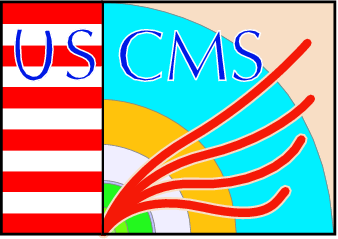
\includegraphics[height=0.6cm]{../../../Graphics/USCMS_logo.png}\hspace{.1cm}
\includegraphics[height=0.75cm]{../../../Graphics/UW_logo.png}}

\begin{document}

\begin{frame}
    \titlepage
\end{frame}

%\section{Overview}
%\begin{frame}
%    \tableofcontents
%\end{frame}

\section{Facilities}
\subsection{Software and Storage}
\begin{frame}
\frametitle{}
\begin{itemize}
    \item Most dCache discrepancies are transient (resolved within hours)
    \begin{itemize}
        \item Decreased monitor sensitivity to filter out harmless cases
    \end{itemize}
    \item PNFSManager ran out of disk space 2008.11.24; remounted PNFS nodes and restarted dCacheDomain
    \item CMSSW\_2\_0\_12 corrupted 2008.11.23
    \begin{itemize}
        \item Redundant copies of CMSSW to improve reliability
        \item Post-installation copy operation fixes hardcoded paths
        \item CMSSW\_2\_0\_X creates {\tt ToolCache.db}, which doesn't like getting fixed
        \item Earlier versions had a flat text file; later versions gzip the file
        \item Disabled path fixing for now, but need to come up with another approach
    \end{itemize}
    \item Still investigating rogue jobs on gatekeeper
    \item Cleaned up OSG accounts and GUMS-to-OSG mappings
    \begin{itemize}
        \item Including loose mapping which allowed OSG VO jobs to run as osg\_mis on gatekeeper
    \end{itemize}
    \item Brief (planned) cooling outage on 2008.11.17; shut down hottest racks
    \item Expanded login pool
\end{itemize}
\end{frame}

\subsection{Production and Monitoring}
\begin{frame}
\frametitle{}
\begin{itemize}
     \item JobRobot:
     \begin{itemize}
        \item Errors due to CMSSW\_2\_0\_12 corruption and transient file errors
     \end{itemize}
     \item SAM:
     \begin{itemize}
        \item More CMSSW errors
     \end{itemize}
     \item RSV: OK
     \item PhEDEx:
     \begin{itemize}
        \item 3\_0\_6 is working fine
        \item Usual MC sample subscriptions for local users and LoadTest activity in the Debug instance.
     \end{itemize}
     \item MC Production:
     \begin{itemize}
        \item Summer08 production continues\ldots{}
     \end{itemize}
\end{itemize}
\end{frame}

\end{document}
